\section{Feature Learning}
In this section, we take a re-look at the NTK and NTK matrices, and explicitly write down the terms related to feature learning.\hfill\\
\textbf{ReLU artefact or NTF vs NPF:} Recall that the neural tangent feature is given by $\psi_{x,t}=\phi^\top_{x,t} {\partial} v_t + {\partial} \phi^\top_{x,t} v_t$. We note that, in the case when $A_t(x,p)\in\{0,1\}$ (such as in DNN with ReLU activations)  $\partial_{\phi}=0$, and hence is not accounted for in the SGD update as well as in the trajectory analysis. However, due to the SGD update, the gating value changes during training, and consequently the activations, the NPF, the NPK change during training as seen in the experiments in \Cref{sec:generalisation}. We side step this artefact by studying network with soft-gates: given a pre-activation input, a hard gate (uch as ReLU) uses $\mathbbm{1}_{\{q>0\}}$, while a soft-gate uses a soft-max sigmoidal function $\chi_\epsilon(q)=\frac{1+\epsilon}{1+\exp(-\beta q)}$. We consider sofr-ReLU networks denoted by $\N_{SR}(\Theta_t)$, and soft-GaLU networks denoted by $\N_{G}(\Theta_t, \G(\N_{SR}(\Tg_t)))$. We checked the performance of soft-gates by training, a soft-GaLU network and a soft-ReLU network, and the fact that adaptable gates generalise better than frozen gates continued to hold (see \Cref{fig:gen} which shows the performance of all the $4$ networks namely ReLU, frozen-GaLU, soft-GaLU and soft-ReLU).\hfill\\
\textbf{NTK and feature learning:} In the case of  soft-GaLU networks, since there are two set of parameters (total $2d_{net}$), we have the neural tangent feature to be $\psi_{x,t}=[\psi^v_{x,t},\psi^a_{x,t}]=[\partial_{\Theta} \hat{y}_t, \partial_{\Tg} \hat{y}_t]\in \R^{2d_{net}}$. Thus the NTK matrix is given by $K_t=K^w_t+K^a_t$,  where $K^w_t={\Psi^v_t}^\top \Psi^v_t$, and $K^a_t={\Psi^a_t}^\top \Psi^a_t$, where $\Psi^v_t=[\psi^v_{x_s,t},s\in[n]]$ and $\Psi^v_t=[\psi^a_{x_s,t},s\in[n]]$ are the NTF matices. In the case of  soft-ReLU networks, i.e, $\N_{SR}(\Theta_t)$  it is easy to check that $K_t={K^v_t}+{K^a_t}+{\Psi^v_t}^\top {\Psi^a_t}+{\Psi^a_t}^\top {\Psi^v_t}$.
\begin{definition}\label{def:delta}
For a soft-GaLU networks, using any $i\in[d_{in}]$, define $\delta_t(s,s')\stackrel{def}= \underset{{p\rsa i}}{\sum} \sum_{\tg\in\Tg}\frac{\partial A_{t}(x_s,p)}{\partial \tg} \frac{\partial A_{t}(x_{s'},p)}{\partial \tg}$.
\end{definition}

\begin{lemma} Under \Cref{assmp:main}, in soft-GaLU networks we have: (i) $\E{K_0}=\E{K^w_0}+\E{K^a_0}$, 
 (ii) $\E{K^w_0}=\sigma^{2(d-1)} (x^\top x)\odot \lambda_0$,  (iii) $\E{K^a_0}=\sigma^{2d}  (x^\top x)\odot \delta_0$
\end{lemma}
\textbf{Discussion}: \hfill\\
$1.$ Note that in \Cref{def:delta}, $\delta_t$ contains $\partial A_t(x,p)$ terms as opposed to $A_t(x,p)$ term in $\lambda_t$ defined in \Cref{def:lambda}. For a path $p$, if a path contains gates that are very close to either $0$ or $1$, then $\partial A_t(x,p)$ will be very small. Since $\frac{\partial A_{t}(x_s,p)}{\partial \tg}= \sum_{l=1}^{d-1} \Big(\frac{\partial G_{x_s,\Tg_t}(l,\I_l(p))}{\partial \tg} \Big)\Big(\Pi_{l'\neq l} G_{x_s,\Tg_t}(l',I_{l'}(p))\Big)$, for a path $p$ containing $d-1$ gates close to $1$, and only one gate whose pre-activation input is close to $0$ will have a significant $\partial A_t(x,p)$. \hfill\\
$2.$ Let us take the case of classification with cross-entropy loss. Now, say we have trained till some $T$ epochs with good classification (say close to $100\%$) accuracy. Considering the fact that $\hat{y}_T=\Phi_{\Tg_T}v_{\Theta_T}$, the gradient with respect to $\Tg$ will change the NPF matrix $\Phi_{\Tg_T}$ in such a manner to reduce the loss, i.e., increase the margin of each of the classified examples, subject to the `well-conditioned' ness of $K^a_T$. While this scenario is idealistic, in practice, both $\Tg_t$ as well as $\Theta_t$ change, and we need to understand how the joint optimisation and feature learning happens.\hfill\\
\begin{figure}[h]
\resizebox{\textwidth}{!}{
\begin{tabular}{cccc}
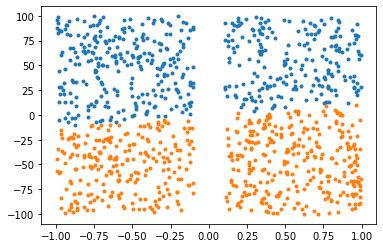
\includegraphics[scale=0.2]{figs/simple-original.png}
&
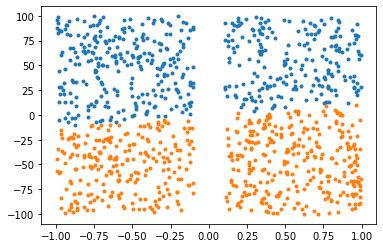
\includegraphics[scale=0.2]{figs/simple-feat.png}
&
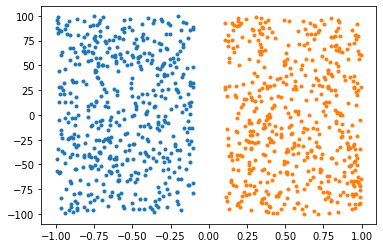
\includegraphics[scale=0.2]{figs/adapt-original.png}
&
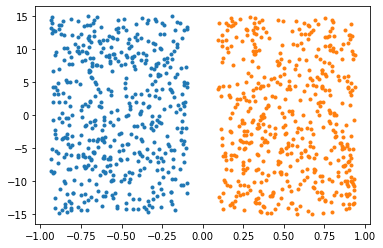
\includegraphics[scale=0.2]{figs/adapt-feat.png}
\end{tabular}
}
\caption{From the left: First two plots show the performance on the original training set with original ($x_s$) and internal feature ($\phi_{x_s,t}$) in the case of frozen-gates. The third and fourth plots show performance on the original ($x_s$) and internal feature ($\phi_{x_s,t}$)  in the case of adaptable gates.}
\label{fig:feat}
\end{figure}

\textbf{Toy Experiment:} We check the performance of frozen-gates versus adaptable gates in a toy experiment. The dataset is $(x_s,y_s)_{s=1}^{n},n=1000$, wherein, for $s=,1,\ldots,500$, $x_s(1)\stackrel{iid}\sim U[0.1,1]$, and $x_s(2)\stackrel{iid}\sim U[-100,100]$, and $y_s=1$, and for $s=501,\ldots,1000$, $x_s(1)\stackrel{iid}\sim U[-0.1,-1]$, and $x_s(2)\stackrel{iid}\sim U[-100,100]$, and $y_s=-1$. We transformed the input $x\in \R^2$ into a feature vector $\phi_{x,t}=(x(1)G_t(1),x(2)G_t(2) )\in \R^2$, where $G_t(i)=\frac{1}{1+\exp(-\tg(i))},i=1,2$. The predicted output is $\hat{y}_{t}(x_s)=\phi^\top_t\Theta_t$, where $\Theta_t\in \R^2$. We use the loss function $L_t=\frac{1}{n}\sum_{s=1}^n\frac{1}{1+exp(-y_s\hat{y}_t(x_s)}$, and trained the model for $T=1000$ epochs, for the following two cases: i) frozen-gates, wherein, we set $\Tg_0=(10,10), \Tg_t=\Tg_0,\forall t\geq 0$, so that the input features are not transformed, and used gradient descent with stepsize $0.1$ to train $\Theta$ ii) adaptable gates, wherein, we performed gradient descent with stepsize equal to $0.1$ to train both $\Tg$ and $\Theta$. The results are shown in \Cref{fig:feat}, notice that the right most plot shows that in the case when the gates are adapting, they learn to suppress the second co-ordinate (the scale of $\phi_{x_s,T}$ is from $-15$ to $15$ as opposed to $-100$ to $100$ in $x_s$). 

\begin{comment}
\textbf{Adaptable gates generalise better:}  On `Binary'-MNIST, we train two more networks namely soft-GaLU and soft-ReLU, where the hard-max in the standard ReLU gating is replaced by a soft-max sigmoid function given by $\chi_{\epsilon}(q)=\frac{1}{1+\exp(-\beta q)}$. In our experiments, we chose $\beta=1$ and $\epsilon=0.1$. The results are shown in \Cref{fig:gen}, where the left most plot shows the optimisation of the $4$ networks (ReLU, frozen-GaLU, soft-ReLU, soft-GaLU), and the middle plot shows the generalisation performance. We can conclude from these plots that adaptable gates generalise better than frozen gates.\hfill\\
\end{comment}
\begin{comment}
\begin{figure}
\centering
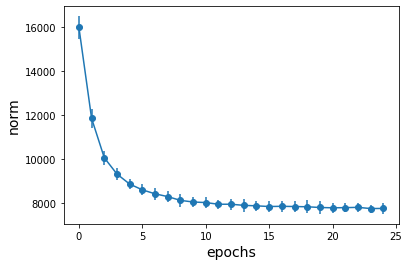
\includegraphics[scale=0.5]{figs/path-gram.png}
\caption{Shows $\nu_t=y^\top (\widehat{M}_t)^{-1}y$, where $H_t=\Phi_t^\top \Phi_t$.}
\label{fig:path-norm}
\end{figure}
\end{comment}

\begin{comment}
\FloatBarrier
\begin{table}[h]
\centering
\resizebox{\columnwidth}{!}{
\begin{tabular}{|c|c|c|}\hline
Terminology& Notation & Remarks\\\hline
ReLU & $\N(\Theta_t,\infty;\Theta_t)$ & $\Theta_t\in \R^{d_{net}}$\\\hline
GaLU (Frozen) &$\N(\Tg_{\dagger},\infty;\Tv_t)$ & $\Tv_t\in \R^{d_{net}}$, $\Tg_{\dagger}\in \R^{d_{net}}$\\\hline
Soft-ReLU &$\N(\Theta_t,\beta;\Theta_t)$ & $G\in(0,1)$ (not decoupled)\\\hline
Soft-GaLU &$\N(\Tg_t,\beta;\Tv_t)$ &  $G\in(0,1)$ (decoupled) \\\hline
\end{tabular}
}
\caption{Shows the variants of DGNs in the experiments. Here, $\dagger$ stands for frozen weights that are initialised by not trained.}% In all our experiments (expect one) we set $\epsilon=0$ in $\chi_{\epsilon}$.}
\label{tb:dgn-family}
\end{table}
\end{comment}

\begin{comment}
\begin{figure*}
\resizebox{\textwidth}{!}{
\begin{tabular}{cccc}
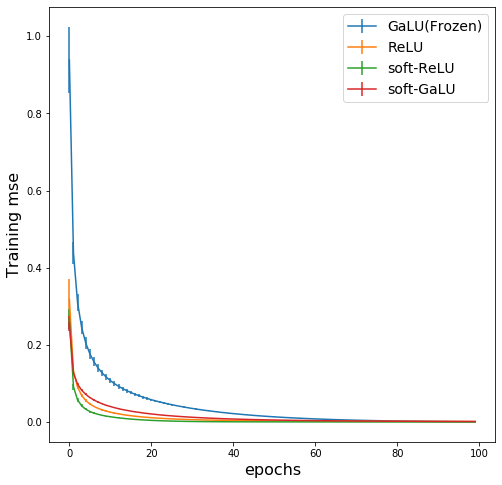
\includegraphics[scale=0.1]{figs/allnet-train.png}
&
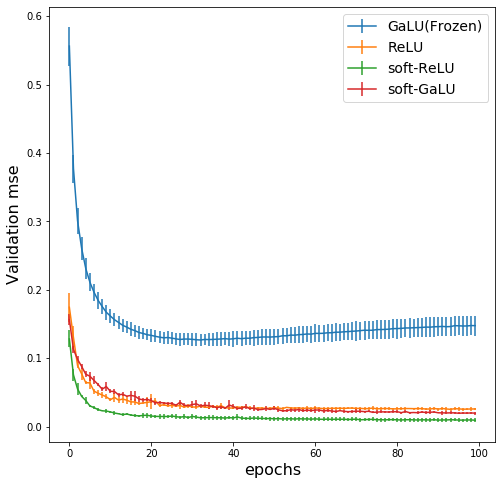
\includegraphics[scale=0.1]{figs/allnet-gen.png}
&
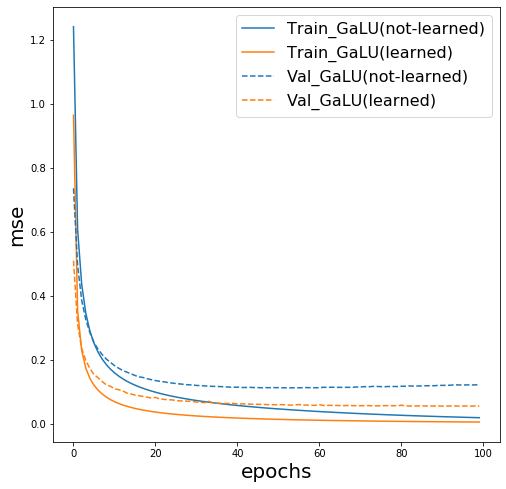
\includegraphics[scale=0.1]{figs/galu-learn-no-learn.png}
&
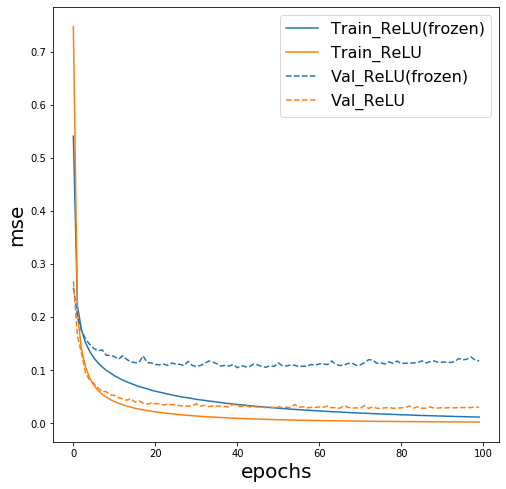
\includegraphics[scale=0.1]{figs/relu-froze-no-froze.png}

\end{tabular}
}
\caption{The left two plots show respectively the training and generalisation in the $4$ different networks with $w=100$, $d=6$. Generalisation performance (dotted lines) of learned gates vs unlearned gates ($3^{rd}$ from left), adaptable gates vs frozen gates (rightmost). The plots are averaged over $5$ runs. }
\label{fig:adapt}
\end{figure*}

\begin{figure*}
\resizebox{\textwidth}{!}{
\begin{tabular}{ccccc}
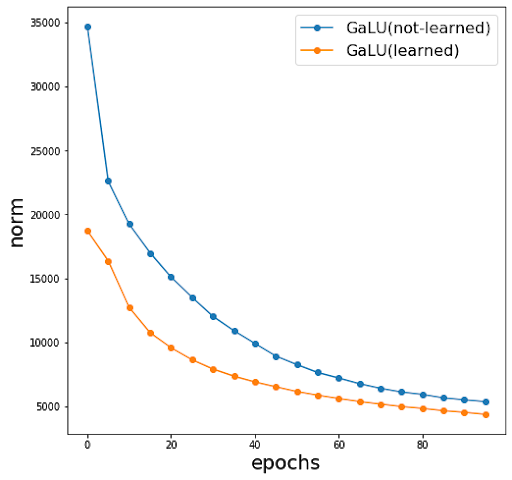
\includegraphics[scale=0.1]{figs/galu-learn-no-learn-knorm.png}
&
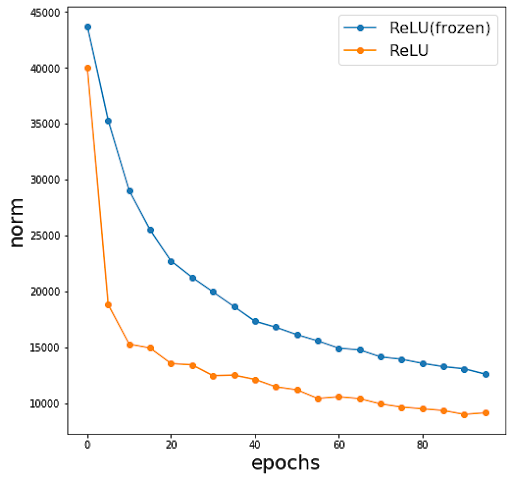
\includegraphics[scale=0.1]{figs/relu-froze-no-froze-knorm.png}
&
%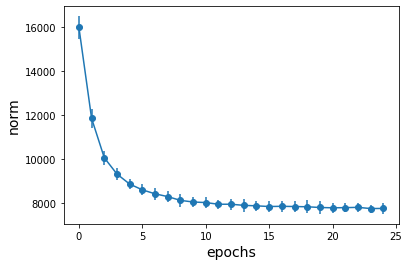
\includegraphics[scale=0.18]{figs/path-gram.png}

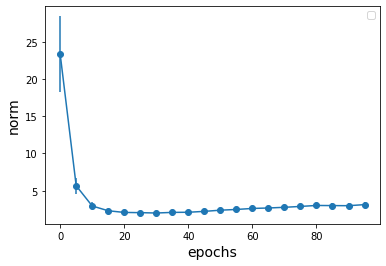
\includegraphics[scale=0.18]{figs/activation-gram-unnorm.png}
&
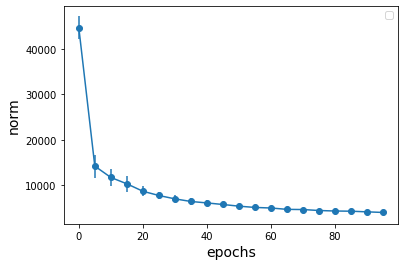
\includegraphics[scale=0.18]{figs/activation-gram-norm.png}
\end{tabular}
}
\caption{Shows $\nu_t=y^\top (H_t)^{-1}y$ for (from the left) i) $H_t=\widehat{K}_t$, ii) $H_t=\widehat{K}_t$,  (iii) $H_t=K^a_t$ (iv) $H_t=\widehat{K^a_t}$. Here $K^a_t$ is the Gram matrix of activations in the soft-GaLU network.}
\label{fig:adapt-norm}
\end{figure*}
\end{comment}
\begin{comment}

We now explain the idea behind the various gates (and some more) in \Cref{tb:dgn-family} as follows:

$1.$ The most general gate is called the \emph{soft-GaLU} gate denoted by $\N(\Tg,\beta;\Tv)$. Here, the gating values and hence the path activation levels are decided by $\Tg_t\in\R^{d_{net}}$, and the path strengths are decided by $\Tv_t\in \R^{d_{net}}$. This network has $2d_{net}$ parameters. % Both $\Tg_0$ and $\Tv_0$ are independent of each other and initialised according to Assumption~\ref{assmp:mainone}.

$2.$ The standard DNN with ReLU gating is denoted by $\N(\Theta_t,\infty;\Theta_t)$, where $\infty$ signifies that the outputs are $0/1$ (see \Cref{tb:dgn-parameterised}). Here, both the gating (and hence path activation levels) and the path strengths are decided by the same parameter namely $\Theta_t\in\R^{d_{net}}$.

$3.$ $\N(\Theta_t,\beta;\Theta_t)$ is a DNN with what we call the \emph{soft-ReLU} gates, where the gating values are in $(0,1+\epsilon)$ instead of $0/1$. Here too, like the standard ReLU networks, both the gating values and the path strengths are decided by $\Theta_t\in\R^{d_{net}}$.

$4.$ $\N(\Tg_{\dagger}, \infty;\Tv_t)$ is what we call a GaLU-frozen DGN, where the gating parameters $\Tg\in \R^{d_{net}}$ are initialised but not trained. 

$5.$ $\N(\Tg_t,\beta;\Tv_{\dagger})$ is a network where only the gating parameters $\Tg_t\in \R^{d_{net}}$ are trainable and the parameters which dictate the path strengths namely $\Tv$ are initialised by not trained.

\end{comment}

\begin{comment}
%In contrast, the `soft-gating' is differentiable, and hence if follows that $\frac{\partial \phi_{x_s,\G_t }^\top}{\partial \theta(m)} w_{t}\neq 0$, which is also accounted in the analysis.
 \textbf{Soft-Gating}: We refer to the function $\chi_\epsilon(v)$ in \Cref{tb:dgn-parameterised} as the \emph{soft} gating function, which takes values in $(0,1+\epsilon)$.  An important feature of the soft-gate is that, the term $\frac{\partial \phi_{x_s,\G_t }^\top}{\partial \theta(m)} w_{t}\neq 0$, which is accounted in both analysis as well as the gradient descent update rule.
 
 
\textbf{Gram Matrices with gate adaptation term:} In the case of $\N(\Tg_t,\beta;\Tv_t)$ networks (which we call as soft-GaLU networks), since there are two set of parameters (total $2d_{net}$) $\Psi_t^\top=[{\Psi^w}^\top_t,{\Psi^a}^\top_t]$ is a $n\times 2d_{net}$, we have $K_t=K^w_t+K^a_t$,  where $K^w_t={\Psi^w_t}^\top \Psi^w_t$, and $K^a_t={\Psi^a_t}^\top \Psi^a_t$. In the case of $\N(\Theta_t,\beta;\Theta_t)$ (which we call as soft-ReLU)  we have $K_t={K^w_t}+{K^a_t}+{\Psi^w_t}^\top {\Psi^a_t}+{\Psi^a_t}^\top {\Psi^w_t}$.

\begin{definition} 
For a soft-GaLU DGN, using any $i\in[d_{in}]$, define $\delta(s,s')\stackrel{def}= \underset{{p\rsa i}}{\sum} \sum_{m=1}^{d_{net}}\frac{\partial A_{\Tg_0}(x_s,p)}{\partial \tg(m)} \frac{\partial A_{\Tg_0}(x_{s'},p)}{\partial \tg(m)}$.
\end{definition}

\begin{lemma} Under \Cref{assmp:main}, in soft-GaLU networks we have: (i) $\E{K_0}=\E{K^w_0}+\E{K^a_0}$, 
 (ii) $\E{K^w_0}=\sigma^{2(d-1)} (x^\top x)\odot \lambda$,  (iii) $\E{K^a_0}=\sigma^{2d}  (x^\top x)\odot \delta$
\end{lemma}
\end{comment}
\begin{comment}
Recall that $\G_t\stackrel{def}=\{G_{x_{s},t}(l,i) \in [0,1], \forall s\in[n],l\in[d-1],i\in[w]\}$. We now define the following:

$\bullet$ \textbf{Active Gates:} For an input $x_{s}\in \R^{d_{in}}$, and a threshold value $\tau_{\A}\in (0,1+\epsilon)$, define $\G_t^{\A}(x_s,\tau_{\A})\stackrel{def}=\left\{G_{x_s,t}(l,i)\colon G_{x_s,t}(l,i)> \tau_{\A}, l\in[d-1],i\in[w]\right\}$. These are the gates that are \emph{on} (i.e., more than threshold $\tau_{\A}$) for input $x_s\in\R^{d_{in}}$.

$\bullet$ \textbf{Sensitive Gates:} For an input $x_{s}\in \R^{d_{in}}$, and a threshold value $\tau_{\S}>0$, define $\G_{t}^{\S}(x_s,\tau_{\S})\stackrel{def}=\cup_{m=1}^{d_{net}}\left\{G_{x_s,t}(l,i)\colon \left|\frac{\partial G_{x_s,t}(l,i)}{\partial \tg(m)}\right| >\tau_{\S},l\in[d-1],i\in[w] \right\}$. These are set of gates that are sensitive to changes in anyone of the $\tg(m),m\in[d_{net}]$ tunable parameters that control the gates.

$\bullet$ \textbf{Relation between sensitive and active gates:} From the nature of the soft-gating function $\chi_{\epsilon}(v)$ it follows that for any given $\tau_{\A}\in(0,1+\epsilon)$, it follows that $\G_t^{\A}(x_s,\tau_{\A})\cap \G_t^{\S}(x_s,\tau_{\S})=\emptyset,\forall \tau_{\S}>\frac{d \chi_{\epsilon}(v)}{d v}|_{v=\chi^{-1}_{\epsilon}(\tau_{\A})}$. Also, note that as $\tau_{\A}\ra (1+\epsilon)$, $\tau_{\S}\ra 0$.

$\bullet$ \textbf{Sensitivity of Activations:} For a path $p$, and a gating parameter $\tg(m),m\in[d_{net}]$ we have $\frac{\partial A_{\Tg_t}(x_s,p)}{\partial \tg(m)}$ to be equal to
\begin{align}\label{eq:sensitivity}
\sum_{l=1}^{d-1} \Big(\frac{\partial G_{x_s,\Tg_t}(l,p(l))}{\partial \tg(m)} \Big)\Big(\Pi_{l'\neq l} G_{x_s,\Tg_t}(l',p(l'))\Big)
\end{align}

In what follows we assume that $\tau_{\S}>\frac{d \chi_{\epsilon}(v)}{d v}|_{v=\chi^{-1}_{\epsilon}(\tau_{\A})}$.

$\bullet$ \textbf{Active Sub-Network:} Which paths are active for input $x_s\in\R^{d_{in}}$?\quad Choose a threshold $\tau_{\A}$ close to $1$. The paths that pass through gates in $\G_t^{\A}(x_s,\tau_{\A})$ do not matter much in gate adaptation because they are already \emph{on}, and are responsible for holding the memory for input $x_s\in\R^{d_{in}}$. In particular, \eqref{eq:sensitivity} evaluates close to $0$ for such paths because $\left|\frac{\partial G_{x_s,\Tg_t}(l,p(l))}{\partial \tg(m)}\right|<\frac{d \chi_{\epsilon}(v)}{d v}|_{v=\chi^{-1}_{\epsilon}(\tau_{\A})}$.

$\bullet$ \textbf{Sensitive Sub-Network:} Which paths are learning for input $x_s\in\R^{d_{in}}$? \quad Those paths that have one gate from $\G^{\S}_t(x_s,\tau_{\S})$ and the rest of the $(d-2)$ gates from the set  $\G^{\A}_t(x_s,\tau_{\A})$. For such paths, the magnitude of at least one of the $(d-1)$ terms in \eqref{eq:sensitivity} will be greater than $\tau_{\S}(\tau_{A})^{(d-2)}$, and the rest of the $(d-2)$ terms will contain a term whose magnitude is less than $\frac{d \chi_{\epsilon}(v)}{d v}|_{v=\chi^{-1}_{\epsilon}(\tau_{\A})}$ component and hence will contribute less to the summation.

$\bullet$ \textbf{Role of $\beta$} for now is limited to an analytical convenience, especially to address the non-differentiability artefact in ReLU gates. The ideas is that as $\beta\ra\infty$, the analysis applies more sharply to networks with ReLU gates.

\end{comment}